%% LyX 2.0.6 created this file.  For more info, see http://www.lyx.org/.
%% Do not edit unless you really know what you are doing.
\documentclass[english]{article}
\usepackage[T1]{fontenc}
\usepackage[utf8]{luainputenc}
\usepackage{babel}
\usepackage{graphicx}
\usepackage[unicode=true]
 {hyperref}

\makeatletter

%%%%%%%%%%%%%%%%%%%%%%%%%%%%%% LyX specific LaTeX commands.
%% Because html converters don't know tabularnewline
\providecommand{\tabularnewline}{\\}

\makeatother

\begin{document}
\title{Spring 2013\\Big Data Final Project\\Parallelize Regularized Greedy Forests}
\author{Hao Liu, Siyuan Zhou}
\maketitle


\section{Overview }

The Regularized Greedy Forest (RGF)\cite{1} is a new decision tree(forest)
method proposed in 2011, which works well in some cases and better
than some well-knowm methods such as, Random Forest, Gradient Boosted
Decision Tree. Our project is to make the trainning process parallel
and scalable by Allreduce\cite{2} on Hadoop.


There are already some good algorithms designed to make decision tree
scalable, such as SLIQ, Sprint and RainForest\cite{4}. And there
are two ways to make it scalable:
\begin{itemize}
\item Sample divide: each subdataset contains some samples of whole dataset
with all features
\item Feature divide: each subdataset contains some features of whole dataset
with all samples
\end{itemize}
We choose sample divide in our program, and make around 4.8 times
speed up on hadoop cluster with 8-15 mappers., but with a small accuracy
drop.


\section{Details}

\subsection{Regularized Greedy Forest }

The Regularized Greedy Forest method can be seen as a combination
of Fully-Correctice Gradient Boosting\cite{1} and Structure Sparsity
Regularization. There are three big differences in RGF:
\begin{itemize}
\item Using the underlying forest structure: While most of the boosting
method using the weak learner as a black box, the RGF using the property
of the weak learner to train the model and optimize the loss function.
Acutally it gives a weight to each leaf in the forest. 
\item Structure Regularization: RGF redefines the loss function to be optimized
by adding a regularization term to original loss function. And this
regularization term will depend on the structure of the forest, such
as the depth of trees and the weights of leaves.
\item Fully Corrective: RGF uses the idea of Fully-Corrective Gradient Boosting\cite{3}
to train the forest. During the tree growing process, RGF optimize
the weights of all leaves, not like the Ada-Boosting or Greedy Boosting
only optimize the weight of last weak learner.
\end{itemize}
Here is the RGF method:
????


\subsection{Scalability by Hadoop and Allreduce}

To solve the aforementioned problem and speed up the training process
of RGF, we use Mapreduce/Hadoop to make it scalable. In the programing
schema of Mapreduce, the data is spreaded among all machines within
a cluster and all processes are isolated from each other, making the
Mapreduce framework the only way of communication. The first assumption
about data is very natural for our problem, where the dataset is line
oriented. But in RGF algorithm, it is necessary to iterate over all
dataset sometime, like finding the best split point in a tree, which
involves trying all possible split points between every pair of adjacent
examples belonging to a given node. Thus communication is unavoidable
with distributed dataset. We have to decouple the algorithm logic
in RGF algorithm where iteration over all dataset is necessary and
allow all processes to communicate to others.


\subsection{Where to do Allreduce }

Fortunately, the communication pattern is simple so that Allreduce
is sufficient for our problem. Concretely, there are two kinds of
unavoided iterations over all dataset in the RGF with L2 regulation:
\begin{itemize}
\item To find the best split (node, feature, threshold), we need to go through
the whole dataset on each node to collect some statistics.
\item To optimize the weights, we need the gradient values of loss function,
which need the whole dataset.
\end{itemize}
Allreduce is used here to get the overall statistics of dataset and
also to get the loss function for whole dataset. Figure~\ref{fig:diagram}is the flow
diagram of the whole pogram:

\begin{figure}
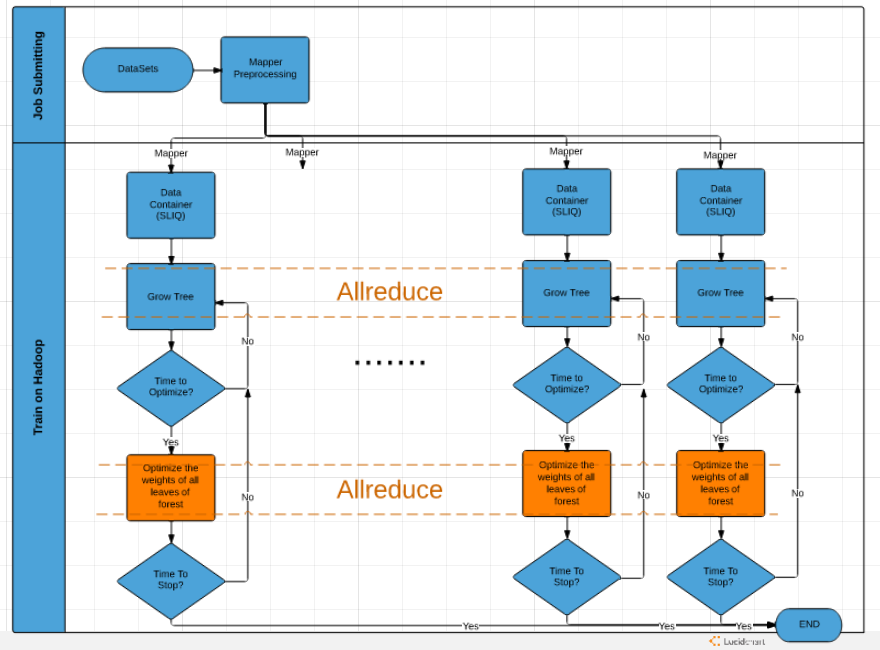
\includegraphics[scale=0.5]{pasted1}
\caption{Fow Diagram} 
\label{fig:diagram}
\end{figure}

The Allreduces of optimization part are very short, like one double
variable, and frequently. So it only takes a very short time. And
the Allreduces in grow tree part are always very expensive. So it
is better if we can make the size and frequency of Allreduce in that
part small. 
\begin{enumerate}
\item For size, the trick is to search the feature bin by bin (quantile)
instead of sample by sample so that we only need to Allreduce the
split points of bin we search. This also make the Allreduce possible
here, because the number of samples arriving each node is different
between mappers.
\item For frequency, the optimal way is to have only two Allreduce in each
tree growing step. But this will greatly destroy the structure of
original code. So we decide to make two allreduces in each tree node:

\begin{itemize}
\item Splits points synchronization: before the search best split (feature,
threshold) pair on each node, for each feature we compute some quantiles
of samples arriving this node and average them over the mappers using
Allreduce.
\item After going through all the split points and collect many statistics,
we make an Allreduce to make 
\end{itemize}
\end{enumerate}

\subsection{Quantile estimation}

Because we are searching through the dataset bin by bin to find the
best threshold for each feature, how to get the bins' split points
is very important. This will decide the accuracy of the method. To
get the split points we need to estimate the quantile of samples arriving
the node we are working on. There are many quantile estimation method
available. 

Suppose we are finding the $p$ quantile, $p\in(0,1)$, and for the
feature we are woring on we have sorted sample set:

$ $
\[
x_{1},\ x_{2},\ ....,\ x_{k}
\]
 Then the simplest way to estimate the quantile is:
\[
Q_{p}=x_{round(p)}
\]


But this is known not stable, sometimes create some strange result,
so we use one of Hyndman and Fan methods, which are robust L-estimators:

$ $
\[
Q_{p}=x_{\lfloor h\rfloor}+(h-\lfloor h\rfloor)(x_{\lfloor h\rfloor+1}-x_{\lfloor h\rfloor}),\ where\ h=(k+1/3)p+1/3
\]


This actually is an interpolation of two datapoint near the quantile. 


\subsection{Visualization:}

We visualize(Figure~\ref{fig:vis}) the train process to show the speed up. It is based on
\href{http://ubietylab.net/ubigraph/}{http://ubietylab.net/ubigraph/}.
The code is available in the cluster/vis.py on hadoop branch.

\begin{figure}
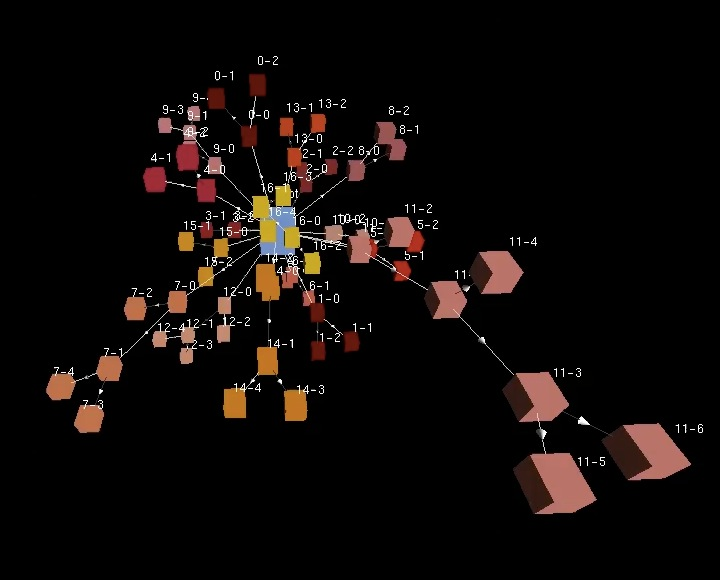
\includegraphics[scale=0.2]{pasted5}
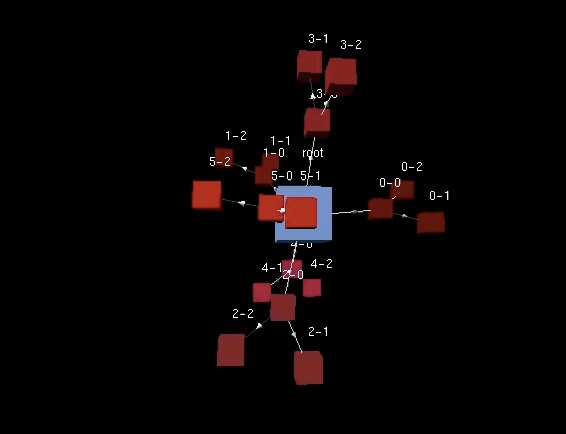
\includegraphics[scale=0.26]{pasted6}
\caption{Visualization} 
\label{fig:vis}
\end{figure}

\section{Experiments:}
In our experiments, we use the dataset \href{http://archive.ics.uci.edu/ml/datasets/Relative+location+of+CT+slices+on+axial+axis}{CT slices}
from the UCI repository. This is a regression problem, so we compare
the accuracy be root mean square error (RMSE).


\subsection{Speed up and time:}

To test speed up rate of our parallel method, we use a dataset of
400MB by duplicating the CT slices many times to simulating the possible
duplication in the real big dataset. And we find around 4.8 times (Figure~\ref{fig:Speedup})
speed up with 100 splits points.

\begin{figure}
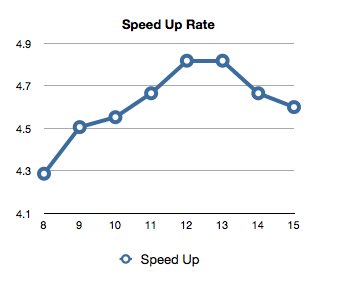
\includegraphics[scale=0.8]{pasted2}
\caption{Speed Up Rate on the number of mappers}
\label{fig:Speedup}
\end{figure}

\textbf{Note }we find there are too much time spent on Allreduce.
But why?
\begin{itemize}
\item Waiting for slow machine? It looks not true: 

\begin{itemize}
\item Figure-1a shows that the Allreduce time grow almost linear when the
number of split points grow, which will only lead the data transferd
by Allreduce change.
\end{itemize}
\end{itemize}

\begin{figure}
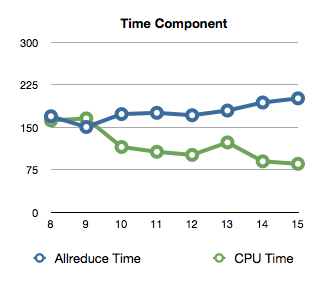
\includegraphics[scale=0.8]{pasted3}
\caption{Time components on the number of mappers}
\label{fig:components}
\end{figure}

\begin{itemize}
\item The Table ~\ref{tab:Allreduce Time} shows the Allreduce time depends on the mount
of data it transfered:
\end{itemize}

\begin{table}
\begin{center}
\begin{tabular}{cccccc}
\hline 
Num splits points & TotalTime & Allreduce Time  & CPU Time & Allreduce data & Allreduce count\tabularnewline
\hline 
\hline 
100 & 274 & 171.107 & 101.08 & 2475498264 & 49730\tabularnewline
\hline 
200 & 302 & 237.558 & 133.33 & 5002209248 & 49682\tabularnewline
\hline 
300 & 469 & 331.811 & 154.78 & 7548282720 & 49680\tabularnewline
\hline 
400 & 598 & 447.821 & 218.02 & 10124462272 & 49738\tabularnewline
\hline 
\end{tabular}
\caption{Allreduce Time}
\end{center}
\label{tab:Allreduce Time}
\end{table}
\begin{itemize}
\item The Figure \ref{fig:components} shows that the Allreduce time also depends on
the number of mappers, but very slow:

\end{itemize}

\subsection{Error:}

The accuracy of RGF is hurted by the number of split points. And we
test on the local machine (it always crash on the Hadoop sever) that
when we use 1000 split points, the result is as good as original one(Table~\ref{tab:RMSE}).
So how to make it possible on Hadoop server will be the future work.

\begin{table}
\begin{center}
\begin{tabular}{ccc}
\hline 
Num of leaves & Original RMSE & 1000 Split Points RMSE\tabularnewline
\hline 
\hline 
100 & 12.25 & 12.61\tabularnewline
\hline 
200 & 10.16 & 10.16\tabularnewline
\hline 
300 & 9.486 & 9.361\tabularnewline
\hline 
400 & 8.907 & 8.862\tabularnewline
\hline 
500 & 8.582 & 8.586\tabularnewline
\hline 
\end{tabular}
\caption{The RMSE on number of leaves}
\end{center}
\label{tab:RMSE}
\end{table}


\subsection{Code on github:}

The code on \href{https://github.com/ylyhlh/RGF_Hadoop}{https://github.com/ylyhlh/RGF\_{}Hadoop}.
And the branch hadoop is what we are working with on Hadoop system.


\subsection{Future Work / Conclusion}
\begin{thebibliography}{1}
\bibitem[1]{1}Rie Johnson and Tong Zhang. Learning nonlinear functions
using regularized greedy forest. Technical report, Tech Report: arXiv:1109.0887,
2011.

\bibitem[2]{2}Alekh Agarwal, Olivier Chapelle, Miroslav Dud'ık, John
Langford A Reliable Effective Terascale Linear Learning System CoRR,
Vol. abs/1110.4198, 2011.

\bibitem[3]{3}Shai Shalev-Shwartz, Nathan Srebro, and Tong Zhang.
Trading accuracy for sparsity in optimization problems with sparsity
constraints. Siam Journal on Optimization, 20:2807–2832, 2010.

\bibitem[4]{4}Johannes Gehrke and Raghu Ramakrishnan and Venkatesh
Ganti RainForest - a Framework for Fast Decision Tree Construction
of Large Datasets In VLDB, 1998.\end{thebibliography}

\end{document}
